El modelo de E/S impulsado por eventos sin bloqueo le brinda a NodeJS un rendimiento muy atractivo, superando fácilmente los entornos de servidores como PHP y Ruby on Rails, que bloquean las E/S y manejan múltiples usuarios simultáneos en hilos separados para cada uno. Algo importante que se debe saber es que NodeJS no es un framework sino un entorno, hay frameworks que funcionan con Node, como Express y Sails, lo que facilita la creación de aplicaciones.
\vspace{0.8cm}

\begin{figure}[H]
  \centering
  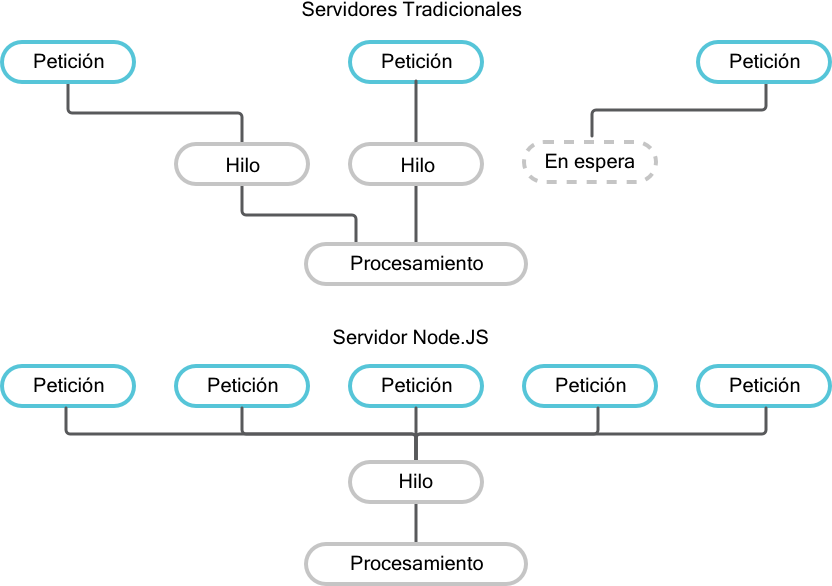
\includegraphics[width=0.8\textwidth]{node-traditional}
  \caption{Comparación de node y servidores tradicionales.}
\end{figure}

Un servidor Node.js tiene un solo subproceso de bucle de eventos (event-loop) que espera E/S en sockets y archivos. Una vez que los datos están listos, activa el método de evento correspondiente y espera hasta que regrese antes de esperar nuevamente por más eventos de E/S. Dado que todas las operaciones de E/S no bloquean, se asegurará de que todo se ejecute correctamente tan pronto como la entrada esté disponible sin ningún bloqueo y sin que se tenga lidiar con problemas de subprocesos múltiples.

\newpage
\subsubsection{Programación basada en eventos}
La filosofía central detrás de NodeJS es la programación basada en eventos. Significa que, el programador,  debe comprender qué eventos están disponibles y cómo responder a ellos. Muchas personas se introducen en la programación basada en eventos mediante la implementación de una interfaz de usuario: el usuario hace clic en algo y se dispara el `evento clic'. Es una buena metáfora, porque se entiende que el programador no tiene control sobre cuándo, o si el usuario va a hacer clic en algo, por lo que la programación basada en eventos es realmente bastante intuitiva \cite{ethan}.
\vspace{0.8cm}

\lstinputlisting[label={node-server}, style=ES6, caption=Configuración servidor NodeJS básico]{code/node-server.js}
En el ejemplo de código \ref{node-server}, el evento es implícito: el evento que se está manejando es una solicitud HTTP. El método http.createServer toma una función como argumento; esta función se invocará cada vez que se realice una solicitud HTTP. El programa simplemente establece el tipo de contenido en texto sin formato y envía la cadena `Hola, mundo!'.
